\chapter{Conclusion}

\section{Discussion of the achieved results}

It is important to note, that there seems to be no universally accepted evaluation metric of realism. Most of today's generative networks are compared using Inception score~\cite{inception}, however, this is only suitable if one is generating actual images and not the depth image with completely different semantics. Another option researches often use is Amazon's Mechanical Turk, however this suffers from the limitation that it might not be clearly obvious how a ``real'' LiDAR-like image (or reconstructed point cloud) from a GTA or Valeo dataset should look like. To properly evaluate the results, whole pipeline using these refined artificial data is needed which was not in the scope of this thesis. Therefore we performed only qualitative analysis of the results showing the generated images.

If we look at the data shown in the figures \ref{evalcmpg2v} and \ref{evalcmpv2g}, we can safely say that the original GAN does not work in this setting regardless of the self regularization of the generators.

This seems to hold for LSGAN without self-regularization as well, however when self-regularization was added, LSGAN started to perform a lot better, preserving the important intensity information. However, it is safe to say that even without rigorous evaluation metric, WGAN-GP with self-regularization term was the winner. It seems to be able to maintain the important information and to introduce noise similar to the real world noise when transforming from the GTA dataset to Valeo dataset, as seen in the point cloud portion of the results.

The most important part of the results is the fact, that the generator of the WGAN-GP network with the self-regularization loss term is able to distinguish between the different objects in the scene and adds the noise in accordance with the expected noise induced by different objects. This can be visible at the figure \ref{carfigs}, where left figure is the original intensity of the car in the GTA data, right figure is the intensity from the refined intensity by WGAN-GP and center figure is the difference between the two figures scaled by 10. The difference is shown in such a way, that if there was no difference, the color has gray-scale value of 0.5 and if the color is lighter than 0.5, then the original intensity was higher than the converted intensity and vice-versa. As you can see, the car and surrounding road is still distinguishable even in the difference image indicating that the generated difference depends on the semantics of the object in the original image. If you look more closely, you can see that the intensity was {\em lowered} on the car which has reflective surface and {\em raised} on the road which is in accordance with the physical state of the world.

\begin{figure}
\subfloat[Original intensity on the car]{
\includegraphics[keepaspectratio, width=0.3\linewidth]{img/carorig.png}}
\hfil
\subfloat[Difference of intensities]{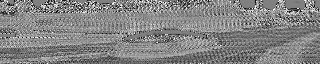
\includegraphics[keepaspectratio, width=0.3\linewidth]{img/cardiff.png}}
\hfil
\subfloat[Refined intensity on the car]{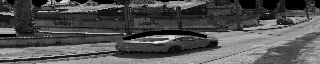
\includegraphics[keepaspectratio, width=0.3\linewidth]{img/carconv.png}}
\caption{Comparison of LiDAR intensities on the car}
\label{carfigs}
\end{figure}

\section{Future work}

In the future we would like to develop a sensible metric for generating depth data. This can be seen as the biggest shortcoming of this thesis. It will be also beneficial to leverage more information from the data in order to be able to create more accurate models of the depth sensors. The most beneficial would be to use RGB data with the LiDAR data simultaneously, however this was not possible due to the missing calibrated RGB images in the Valeo dataset.

It might be interesting to explore the idea of asymmetric CycleGAN in which the generators' structures as well as the input and output shapes differ. This use-case can be potentially very interesting as it can lead to using more information from one dataset if available.

\section{Conclusion}

We showed that the generative modeling of LiDAR-like data is feasible in the CycleGAN setting. This is an important result since as far as we know it was never tried before. The results indicate that it is necessary to be extremely careful about used loss functions and underlying generative models used in the CycleGAN. We believe that if more detailed data (namely RGB images corresponding to the LiDAR scans) were available to the training pipeline, achieved results would be even more convincing.
